\documentclass[11pt]{article}
\usepackage[utf8]{inputenc}
\usepackage{longtable}
\usepackage{color}
\usepackage{multirow}
\usepackage{hyperref}
\usepackage{setspace}
%\doublespacing

\renewcommand*{\sectionautorefname}{Section} 

\title{Documentation \_A \\ Policy emergence model}
\author{Raphael Klein}

\usepackage{natbib}
\usepackage{graphicx}
\usepackage[labelfont=bf]{caption} 	% Make captions bold (Figure & Table)
\usepackage{subfig}	
\usepackage{amsmath}
\usepackage{hyperref}
%\usepackage[section]{placeins}

\providecommand{\keywords}[1]{\textbf{Keywords:} #1}

\begin{document}

\maketitle

%\begin{center}
%Word count: 9300 words
%\end{center}

This report documents the conceptualisation and the formalisation of an agent based ACF model.

\tableofcontents

%%%%%%%%%%%%%%%%%%%%%%%%%%%%%%%%
\section{Model conceptualisation}

The policy process model is specified according to the four key elements that were outlined in the literature: time, policy arena, agents and interactions\footnote{Klein, R; Ashkenazy, A.; Nikolic, I.; Bots, P.W.G. "Developing a common language of the policy process for modellers", Policy Studies Journal (under review).}. The main choice that is left to the modeller is to decide how much complexity needs to be integrated to each of these elements to answer the research question. In the present case, only a limited amount of complexity is required. This leads to a relatively simple policymaking process model. It is detailed below.

For the ACF approach, we consider the model with two different levels of complexity - policy learning (PL) and coalitions (Co), and two add-ons - partial knowledge (PK) and partial information (PI). The add-ons are model parts that can be introduced regardless of the level of complexity considered. Throughout this document, we will refer to these four different model parts through their acronyms. This builds on the simplest implementation model\footnote{\url{https://github.com/kleinrap/policyemergence_SM}}.

%%%%%%%%%%%%%%%%
\subsection{Time}

For the time element, no changes are made from the simplest implementation. Two steps are considered: agenda setting and policy formulation.

%%%%%%%%%%%%%%%% end of the time subsection

%%%%%%%%%%%%%%%%
\subsection{The policy arena}

This policy arena is defined in the same way as the simplest implementation as well.

%%%%%%%%%%%%%%%% end of the policy arena subsection

%%%%%%%%%%%%%%%%
\subsection{The agents and the environment}

Again we retain the policy makers, electorate and their belief system. The introduction of the ACF brings a slew of additional elements detailed below.

To emulate policy learning, we introduce policy entrepreneurs. These are agents that have for goals to push forward their interests. They can do so using resources. These resources are defined based on political or economical resources that the actors might have in real life.

To emulate coalitions, we introduce an aggregate agent that is the coalition. These coalitions are made of agents with similar policy core preferred states. They can pool their resources to be more effective throughout the policy process and to push their respective interests.

Finally, the introduction of partial information requires the introduction of an additional agent type: the external party. They are representations of the media, international institutions, academic institutions and NGOs. These are agents that will communicate information from the environment to the rest of the agents in the policy process.

%%%%%%%%%%%%%%%% end of the actors and environment subsection

%%%%%%%%%%%%%%%%
\subsection{The interactions}

The interactions already mentioned for the simplest implementation are kept the same. For each additions related to the ACF, new interactions or changes in the current interactions happen. These are detailed here.

\paragraph{Policy learning}

For policy learning, agent on agent interactions are introduced. Agents can influence one another by targeting other's preferred states and causal beliefs. In effect, this means that the agents can influence each other's goals or their understanding of how the environment works. Agents cannot influence each other's actual beliefs because we assume that the actual beliefs are linked directly to the state of the environment under the assumption of perfect information (this assumption is relaxed for the imperfect information aspects of the model). Agents can only perform one influencing actions at a time. To decide on which action to perform, agents consider all the actions they have at their disposal. They then select the action that is likely to have the most impact based on the average conflict level between agents - agents with an average level of conflict are more likely to interact than with a high or low level of conflict according to the literature.

To limit the amount of interactions and to weigh them depending on the agent's prominence, we introduce the concept of resources. These resources are spent by the agents when they want to influence other agents. When an agent has run out of resources, he is unable to continue influencing other agents. These resources are replenished every round of the policy making process. Only one type of resource is considered, contrary to the literature. We assume that all resources mentioned in the literature, from political resources to public opinion, are aggregated into one resource type for the model.

\paragraph{Coalitions}

The introduction of coalitions also adds new interactions, on top of the newly introduced agent on agent interactions added for policy learning. Coalitions can influence other agents in the same way as any agent would but with additional resources at their disposal. Such influence is aimed at furthering the interests of the coalition - for example achieving their preferred state for the issues around which the coalition has been assembled. This is done by the implementation of policies supported by the coalition. With this in mind, we assume that each coalition can influence either agents within the coalition itself in an effort to increase its cohesion or, agents that are outside the coalition in an effort to implement policies aligned with its interests. We assume that depending on the cohesion of the coalition, it will assign different amount of resources for either cohesion building influence or outside influence. 

Similarly to the agents, the coalition influence can be exercised on the preferred states of other agents or their causal beliefs. The difficulty when implementing such actions within a simulation is to choose who exercises this influence and how the actions are selected. The assumption made is that the influence actions of each coalitions are based on the average of the preferred states or the causal beliefs - depending on the action considered - of the members of the coalition. The actions are then performed in a similar fashion as individual agents, by considering the conflict level. No leader or key figure is then needed.

\paragraph{Partial knowledge}

By considering partial knowledge, we assume that agents only have an approximate understanding of other's beliefs. The only way to gain more knowledge of other's beliefs is to interact with them. By interacting, agents become better aware of one another's beliefs. Overall, introducing partial knowledge means that agents will plan their interactions with a certain amount of uncertainty, leading to potentially ineffective influencing interactions. For example, an agent might try to influence another agent's causal beliefs while both agents have the same causal beliefs. This results in a waste of resources for the first agent. Agents increase their knowledge of other agents' beliefs through interactions to avoid such mistakes being repeated.

\paragraph{Partial information}

We so far assumed that information flowing from the environment into the policymaking process model was perfect. This meant that the actual beliefs of the agents reflect what is happening in the environment. For example, for a policy core issue of crime, if there are 300 crimes per year, this will be the information agents consider when selecting policy instruments. However, in reality, agents often receive imperfect or distorted information. This can be due to the channels they use to inform themselves amongst other things. Aspect of imperfect information can be included in the model as well. We approach this inclusion through the addition of external parties who come with specific new interactions.

We assume that the external parties are the agents that can obtain the real states of the environment and will go on to inform all other agents in the model. Based on their own preferred goals, they will distort the information they are conveying to further their interests. The policy makers and policy entrepreneurs will inform their actual beliefs from the information provided by these external parties.


%%%%%%%%%%%%%%%% end of the interactions subsection
%%%%%%%%%%%%%%%%%%%%%%%%%%%%%%%% end of the model conceptualisation section

%%%%%%%%%%%%%%%%%%%%%%%%%%%%%%%%
\section{Model formalisation (SM)}

In this section we mention only the parts of the model that are common to all of the ACF implementations based on the simplest implementation.

%%%%%%%%%%%%%%%%
\subsection{The process}

The process changes for each of the complexity additions.

%%%%%%%%%%%%%%%% end of the process subsection

%%%%%%%%%%%%%%%%
\subsection{The agents}

There are two main categories of agents in the model: the active agents that have a direct influence on the agenda and the passive agents that have an indirect impact on the agenda and policy change.

%%%%%%
\paragraph{Active agents}

The active agents are the policy makers. Their attributes are given as follows:

\begin{enumerate}

\item The \emph{active agent} is represented as an 6-tuple given by \texttt{agent = (ID, type, beliefHierarchy, affiliation, advocacy, resources)} where
\texttt{ID} is the agent unique ID,
\texttt{type} is the agent type, 
\texttt{beliefHierarchy} is the agent's personalised belief hierarchy, 
\texttt{affiliation} is the political entity the agent identifies with,  
\texttt{advocacy} is the list of the issues the agent is supporting,
\texttt{resources} corresponds to the amount of resources the agents have.

\item A \emph{type} corresponds the agent type: policy maker. This will go on to define the actions possible for the agent.

\item The \emph{affiliation} is used only when the electorate is considered as affiliations help differentiate different groups of agents according to their political leanings.

\item The \emph{belief hierarchy} is made of the agent's own belief hierarchy structure and associated values.

\item The \emph{advocacy} is represented as a 2-tuple \texttt{(issue\_as, issue\_pf)} where \texttt{policy\_as} is the issue chosen by the agent during the agenda setting step, while the \texttt{policy\_pf} is the policy instrument selected by the agent in the policy formulation step.

\end{enumerate}

%%%%%% end of the active agents paragraph


%%%%%%
\paragraph{Passive agents}

The passive agents are the truth agent and the electorate.

\emph{The truth agent:} The truth agent is an agent included only for programming purposes. This agent provides a link between the environment and the policy agents. It is communicated all the states of the environment and informs the actual beliefs of the active agents using these states. The only attribute of the truth agent is the belief hierarchy composed only of actual beliefs for each of the issues.

\emph{The electorate: } The electorate represents the different constituencies. There are as many electorate agents as there are political affiliations. The role of the electorate is to influence the policy makers in their aims. The following defines the attributes of the electorate:

The \emph{electorate} can be given as a 3-tuple written as: \texttt{electorate = (ID, affiliation, beliefHierarchy)} where \texttt{ID} is the unique name of the electorate, \texttt{affiliation} is its associated affiliation and \texttt{beliefHierarchy} is the associated belief hierarchy of the electorate.  The belief hierarchy of the electorate is similar in structure to the one of the truth agent but composed only of preferred states.

%%%%%% end of the passive agents paragraph

%%%%%%
\paragraph{Belief hierarchy}

The belief hierarchy is composed of two main parts: the issues and the causal beliefs. The issues are categorised in multiple layers: the deep core issues (the top layer), the policy core issues (the middle layers) and the secondary issues (the bottom layer). Secondary issues are linked to policy core issues through causal beliefs and similarly for policy core issues and deep core issues. The overall representation of this hierarchy structure is shown in \autoref{fig:Formalisation-04}.

\begin{figure}
\centering
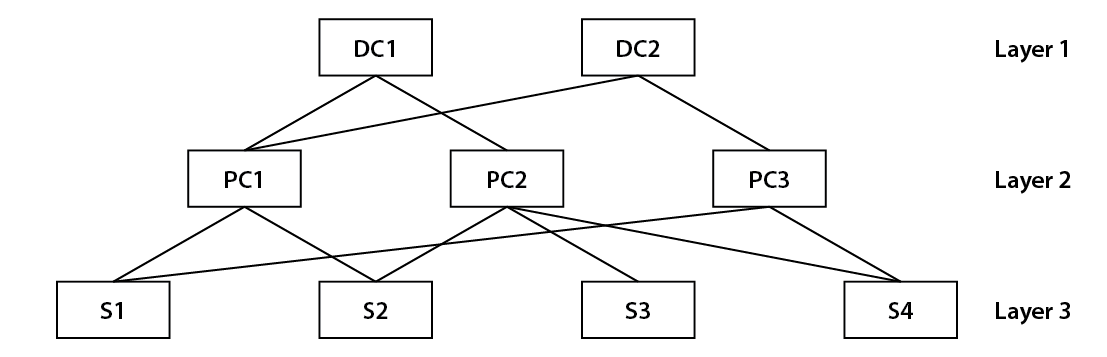
\includegraphics[width = 0.95\linewidth, angle = 0]{figures/Formalisation-04}
\caption{Representation of the belief hierarchy of the agents.}
\label{fig:Formalisation-04}
\end{figure}

Each issue is categorised by three parameters: the actual belief, the preferred state and the preference. The actual belief defines the view of the agent of a certain issue as it is in the environment. They can take values within the interval $[0, 1]$.

The preferred states show where the agent would like the issue be in the future. They can also take values within the interval $[0, 1]$.

The preference is a calculated parameter that defines the urgency that the agent places on the each issues. It is obtained depending on the actual belief, the preferred state and the causal beliefs linked to the issue. Its calculation is detailed later. The sum of all issue preferences on any single layer of the belief hierarchy has to be equal to 1.

The belief hierarchy structure also contains causal beliefs. These can be seen as causal relations. They represent the understanding of an agent about how a change in one issue will lead to a change in another on a different layer. The causal beliefs can take values within the interval $[-1, 1]$. A negative value means that an issue when growing will affect negatively another issue.

%%%%%% end of the belief system paragraph
%%%%%%%%%%%%%%%% end of the agents subsection


%%%%%%%%%%%%%%%%
\subsection{The actions and interactions}

% preferences calculation
% preferences selection
% agenda selection
% policy instrument selection
% electorate influence

There are a number of actions and interactions that the agents can perform. We will first outline the actions that actors have to perform themselves including the calculation of the preferences. We will then outline the agenda and policy instrument selection for the entire policy arena. Finally, we outline how we conceptualise that the electorate influence the policy makers.

%%%%%%
\paragraph{Preference calculation - deep core issues}

For the deep core issues, which are at the top of the belief system, the preferences are calculated differently than for the policy core and secondary issues. The calculation of the preference for each issue is given by:

\begin{equation}
P_i = \frac{ |G_i - B_i|}{\sum_{j=1}^n |G_j - B_j|}
\end{equation}

where $P$ is the preference, $G$ is the preferred state - or Goal, $B$ is the actual belief - or Belief, $j$ is defined as the number of principle belief issues and $i$ is the deep core issue.

%%%%%% end of the preference calculation DC issue paragraph

%%%%%%
\paragraph{Preference calculation - policy core and secondary issues}

The preference calculations for the policy core and secondary issues are adapted to include the causal beliefs that link these layers to their directly above layers.

To calculate the preference, the gap between aim and state for the issues is considered along with the impact of the causal relation on the gap of the issue on the above layers. The causal relations are not always helping bridge the gap between the aim and the state of issues on a higher layer. If this is the case, then the causal relations are not considered within the calculation as there effort is counter productive within the mind of the agent. The resulting equation that can be used to calculate the preference for these layers is given by:

\begin{equation}\label{eq:preference2}
P_k = \frac{ |G_k - B_k| + \sum_{j=1}^n |C_{k,j} \left( G_j - B_j \right)|}{\sum_{l=1}^p \left[ |G_l - B_l| + \sum_{j=1}^n \left|C_{l,j} \left( G_{j} - B_{j} \right) \right| \right]}
\end{equation}

The sums only include the terms $|C \cdot \left( G - B \right)|$, if $C$ and $\left( G - B \right)$ have the same sign. If not, these terms are not considered.

Where $p$ is defined as the number of issues on that layer, $k$ characterises the issue being selected for the calculation, $j$ specifies the issues above the layer considered and $C$ represents the causal belief.

Based on these preferences obtained, the agent will select one issue to advocate. In the agenda setting, the agent will select one policy core issue and for the policy formulation, the agent will select a secondary issue. The issue chosen is the one with the highest preference.

%%%%%% end of the preference calculation PC and S issues paragraph

%%%%%%
\paragraph{Agenda selection}

The \emph{agenda} is a 1-tuple given by \texttt{agenda = (issue)} where \texttt{issue} is the policy core issue that is placed on the agenda by all agents.

To constitute the agenda, an issue has to be chosen as a majority issue by all agents in the policy arena. If no majority is obtained on any issue, then the policy formulation cannot happen as no agenda has been selected.

%%%%%% end of the agenda setting paragraph

%%%%%%
\paragraph{Policy instruments}

The policy instruments are measures that are chosen by the policy makers to influence the environment. To select a policy instrument, the active agents assess the impact of each instrument on the secondary issues in their belief hierarchy. These instruments have an impact on the gap between the actual belief and the preferred state of each of these issues. The policy instruments can be described as follows:

\begin{enumerate}
\item A \emph{policy instrument} is represented as a 2-tuple \texttt{(ID, impact)} where \texttt{impact} is related to the impact of the policy on a specific issue.

\item There are as many \emph{impacts} of a policy instrument as there are secondary issues. These impacts provide an information to the agents on how much the secondary issue will change if that instrument is implemented.

\end{enumerate}

%%%%%% end of policy instrument paragraph

%%%%%%
\paragraph{Preference calculation - policy instruments}

The policy makers have to select a policy instrument that they will advocate for. This is based on their preferences for which the calculation is detailed below:

\begin{equation}
P_k = \frac{\sum_{p = 0}^{n} | G_{p} - \left( B_{p} (1 + I_{k,p}) \right) |}{\sum_{q = 0}^{m} \sum_{p = 0}^{n} | G_{p} - \left( B_{p} (1 + I_{q,p}) \right) |}
\end{equation}

where $k$ is the policy instrument for which the preference is calculated, $n$ is the number of secondary issues, $m$ is the number of policy instruments, $I$ is the impact of the instrument on a specific secondary issue.

Once all the preferences have been calculated, the agent will select the instrument with the highest preference as the instrument s/he will advocate for.

%%%%%% end of the preference calculation policy instrument paragraph

%%%%%%
\paragraph{Policy instrument selection and implementation}

The policy makers are the agents that can selected a policy instrument at the end of the policy formulation step. This is done through a majority vote. If a majority of actors decide on one policy instrument, then that instrument is implemented.

%%%%%% end of policy instrument implementation paragraph

%%%%%%
\paragraph{Electorate passive action on policy makers}

The policy makers are passively influenced by the electorate. Each electorate has a certain affiliation to which policy makers are also related. Each policy makers' issue preferred state will be influenced by their respective electorate. This happens as a passive effect where the preferred states of the policy makers slowly progress towards the issue aims of the electorate. The equation to calculate the change in the aim of the policy maker is given as follows:

\begin{equation}
G_{k} := G_{k} + \left(G_{El} - G_{k} \right) \cdot C_{i}
\end{equation}

where $El$ stands for electorate of same affiliation of the policy maker, $k$ is a policy maker, $C_i$ is a the constant influence that allows variation in the speed of the change of the preferred states of the agents.

%%%%%% end of the electorate action paragraph
%%%%%%%%%%%%%%%% end of the actions and interactions subsection
%%%%%%%%%%%%%%%%%%%%%%%%%%%%%%%% end of the formalisation (SM) section


%%%%%%%%%%%%%%%%%%%%%%%%%%%%%%%%
\section{Model formalisation (+PL)}

In this section we present the model formalisation needed when the policy learning is emulated.

%%%%%%%%%%%%%%%%
\subsection{The process}

Through the introduction of policy learning, a number of additions need to be considered for the process followed. It remains a two-step process. First the agenda setting step is performed, then, if an agenda has been agreed on, comes the policy formulation step. This does not include the environment simulation. The process is detailed below:

\begin{enumerate}
\item Initialisation:
	
	\begin{enumerate}
	\item \emph{Trigger of external events:} Any event that the modeller decides to implement are activated at this stage of the model cycle.
	\item \emph{Update of the truth agent:} Information from the environment is used to inform the truth agent actual beliefs.
	\item \emph{Electorate actions on policy makers} (when included)
	\item \emph{Transmission of the actual beliefs:} The agents are informed about the environment from the truth agent.
	\end{enumerate}
	
\item Agenda setting step:
	\begin{enumerate}
	\item \emph{Resources distribution}
	\item \emph{Preferences calculation (issues):} Each agent calculates the preference for their deep core and policy core issues. Additionally, each agents selects an issue that s/he will advocate for in his/her policy core issues based on the preferences.
	\item \emph{Agent interactions:} The agents influence one another to advance their interest relating to the policy core issues, spending all of their resources.
	\item \emph{Preferences calculation - policy makers (issues):} Policy makers update their preferences before the selection of the agenda to take into account the changes related to the agent interactions.
	\item \emph{Agenda selection}
	\end{enumerate}
	
\item Policy formulation step:
	\begin{enumerate}
	\item \emph{Resources distribution}
	\item \emph{Preferences calculation (policy instruments):} All agents update their preferences for their secondary issues and policy instruments based on the issue on the agenda. All agents then selects a policy instrument that s/he will be advocating for.
	\item \emph{Agent interactions:} The agents influence one another to advance their interest relating to the secondary issues, spending all of their resources.
	\item \emph{Preferences calculation - policy makers (policy instruments):} Policy makers update their preferences before the selection of the policy instrument to take into account the agent interactions.
	\item \emph{Policy instrument implementation} 
	\end{enumerate}

\end{enumerate}

%%%%%%%%%%%%%%%% end of the process subsection

%%%%%%%%%%%%%%%%
\subsection{The agents}

One category of active agents is added to the +PL model: the policy entrepreneur. It has the same attributes as the policy makers with the main difference that policy entrepreneurs have no say in the choice of the policy to implement. The rest remains unchanged.

%%%%%%%%%%%%%%%% end of the agents subsection


%%%%%%%%%%%%%%%%
\subsection{The actions and interactions}

% agent on agent interaction.

Only agent on agent interactions are added through the +PL model. This is detailed here. The rest of the actions and interactions remain unchanged from the SM model.

%%%%%%
\paragraph{Agent on agent interactions}

For every step, the agents can interact with one another. These interactions are focused on the causal beliefs and the preferred states. Agents can only interact on the issues they are advocating for and their related causal beliefs. They spend 10\% of their resources for each action.


First, each agent considers all of the actions that it can perform, grading them, and then deciding which actions will be performed depending on the expected impact of that action.

This grade is obtained based on the conflict level between agents for each issue and, simultaneously, the belief difference between the agents. Following the literature, it is assumed that agents with an average conflict level are most likely to interact, followed by a low and then high conflict level. These are established based on ranges of differences. For example, an average conflict level is when the beliefs of two agents are within 0.2 and 0.4 of one another. Low conflict level is when they are within 0.2 of one another and high conflict level is when there is a greater difference than 0.4. If there is more than one average conflict level in the possible interactions, an action is selected randomly to be performed. If there are none, then a low conflict level action is considered, and so on. Within the simulation, a low conflict level is assigned a grade of 0.50, for medium it is 0.75 and for high it is 0.25. Furthermore, the grade is multiplied by the different in beliefs between the agents to differentiate the decision in case where there is the same conflict level with more than one agent.

%To avoid a scattershot approach from the part of the agent influencing, we will assume that the agent will continue influencing the same randomly selected agent (from the conflict level selection) until that agent's conflict level has reduced to low or the influencing agent has run out of resources. This would mean that the agent has successfully influenced his/her target and brought their belief to a level closer to their own. Without this assumption, and because of the three tiered conflict level approach, agents are likely to influence random agents with whom they have an average level of conflict level every time they have the opportunity to interact. We want to avoid that and have agents follow some sort of strategy. 

Once the interaction has been selected, it needs to be performed. This is done using the following equation for a causal belief:

\begin{equation}
C_{m} := C_{m} + (C_{n} - C_{m}). R
\end{equation}

where $C$ stands for causal belief, $R$ for resources, $m$ for the agent being interacted upon and $n$ for the agent performing the interaction.

And similarly for a preferred state interaction:

\begin{equation}
G_{m} := G_{m} + (G_{n} - G_{m}). R
\end{equation}

where $G$ stands for the preferred state.

%%%%%% end of  paragraph

%%%%%%%%%%%%%%%% end of the actions and interactions subsection
%%%%%%%%%%%%%%%%%%%%%%%%%%%%%%%% end of the formalisation (+PL) section


%%%%%%%%%%%%%%%%%%%%%%%%%%%%%%%%
\section{Model formalisation (+Co)}

The model formalisation +Co introduce the concept of coalition. This builds on the +PL model without which coalitions cannot be considered.

%%%%%%%%%%%%%%%%
\subsection{The process}

The introduction of coalitions add a few sub-steps to the process described in the +PL model. This is detailed below:

\begin{enumerate}
\item Initialisation:
	
	\begin{enumerate}
	\item \emph{Trigger of external events}
	\item \emph{Update of the truth agent}
	\item \emph{Electorate actions on policy makers} (when included)
	\item \emph{Transmission of the actual beliefs}
	\item \emph{Coalitions creation}
	\end{enumerate}
	
\item Agenda setting step:
	\begin{enumerate}
	\item \emph{Resources distribution}
	\item \emph{Preferences calculation (issues)}
	\item \emph{Coalition interactions:} The coalitions perform their intra- and inter-influence actions one another to advance their interest relating to the policy core issues, spending all of their resources.
	\item \emph{Agent interactions}
	\item \emph{Preferences calculation - policy makers (issues)}
	\item \emph{Agenda selection}
	\end{enumerate}
	
\item Policy formulation step:
	\begin{enumerate}
	\item \emph{Resources distribution}
	\item \emph{Preferences calculation (policy instruments)}
	\item \emph{Coalition interactions:} The coalitions perform their intra- and inter-influence actions one another to advance their interest relating to the policy instruments, spending all of their resources.
	\item \emph{Agent interactions}
	\item \emph{Preferences calculation - policy makers (policy instruments)}
	\item \emph{Policy instrument implementation} 
	\end{enumerate}

\end{enumerate}

%%%%%%%%%%%%%%%% end of the process subsection

%%%%%%%%%%%%%%%%
\subsection{The agents}

The agents are the same as in the +PL model. The main addition is that of the coalitions. THey are also considered as active agents in the model.

%%%%%%
\paragraph{Coalitions}

The coalitions have the following attributes attributes:

\begin{enumerate}

\item A \emph{coalition} is represented as an 5-tuple given by \texttt{agent = (coID, members, beliefHierarchy, advocacy, resources)} where
\texttt{coID} is the coalition unique ID,
\texttt{members} is the list of agents that are member of the coalition, 
\texttt{beliefHierarchy} is the coalition's aggregate belief hierarchy based on other agent's beliefs, 
\texttt{advocacy} is the list of the issues the coalition is supporting,
\texttt{resources} corresponds to the amount of resources the coalitions has.

\item The \emph{belief hierarchy} is made based on the average of the member agents' belief hierarchies for causal beliefs, preferred states and actual beliefs.

\item Similarly to agents, the \emph{advocacy} is represented as a 2-tuple \texttt{(issue\_as, issue\_pf)} where \texttt{policy\_pf} is the issue chosen by the agent during the agenda setting step, while the \texttt{policy\_pf} is the policy instrument selected by the agent in the policy formulation step.

\item The \emph{resources} are pooled from the members. For the present formalisation, we will assume that each agent provide 50\% of his/her resources to the coalition to which it belongs. 

\end{enumerate}

%%%%%% end of the coalitions paragraph
%%%%%%%%%%%%%%%% end of the agents subsection


%%%%%%%%%%%%%%%%
\subsection{The actions and interactions}

% intra coalition actions
% inter coalition actions

The introduction of coalition leads to some additional interactions between coalitions and agents, they are detailed here.

%%%%%%
\paragraph{Coalition creation}

The coalitions are created surrounding policy core issues where agents have similar preferred states. Often one policy core issue is considered to be critical, this does not change throughout the process. This issue can be chosen prior to the simulation by the modeller.

In the present formalisation, we assume that agents have similar beliefs if they are within 0.3 of one another. Therefore, coalitions are created whenever a number of agents are within 0.3 of one another. Finally, we also assume that there cannot be more than three coalitions and there will often only be two coalitions.

%%%%%% end of the coalition creation paragraph

%%%%%%
\paragraph{Coalition on agent interactions}

In the present formalisation, we assume the following:

\begin{itemize}
\item Coalitions behave like other agents, therefore perform the same interactions.
\item Coalitions can influence their own members.
\item Coalitions can only influence agents individually and not coalitions as whole entities.
\end{itemize}

The coalitions spend some of their resources to increase the coherence between their members. This means spending up to 30\% of their resources on members to make sure that their beliefs are within 0.2 of the coalition average for the issues advocated by the coalition.

The rest of their resources is used to influence external agents. The interactions used are the same as the agent on agent interactions but where the coalition is considered as an agent. For each action, the coalition spends 1\% of its resources.

%%%%%% end of the coalition on agent interactions paragraph
%%%%%%%%%%%%%%%% end of the actions and interactions subsection
%%%%%%%%%%%%%%%%%%%%%%%%%%%%%%%% end of the formalisation (+Co) section


%%%%%%%%%%%%%%%%%%%%%%%%%%%%%%%%
\section{Model formalisation (+PK)}

The introduction of the partial knowledge into the model has no impact on the process or the agents. It only impacts the agent on agent interactions. This is explained below. Note that the +PK model can be added to the SM, the +PL and the +Co models. It will only have an impact on the two latter as the SM does not have any agent interaction to be influence by partial knowledge.

%%%%%%%%%%%%%%%%
\subsection{The actions and interactions}

Changes in the agent on agent interactions are detailed here.

%%%%%%
\paragraph{Agent on agent interactions}

When considering partial knowledge, the actions between the agents are not changed. The main difference is that now the conflict level is calculated based on the knowledge of the agents of other agents' beliefs. This knowledge of other's beliefs is updated after every interaction based on the assumption that through their interactions, both agents gain better knowledge of the beliefs of the other.

The update of this knowledge is performed using the following equation:

\begin{equation}
B_{m} := B_{m} + (B_{n} - B_{m}). W_{gap}
\end{equation}

where $B$ is the belief in question, $m$ is the agent who is updating his knowledge, $n$ is the actual belief of the other agent, $W_{gap}$ is a weighing constant that can be used to scale the speed at which knowledge is acquired through interactions. This equation applies equally for actual beliefs, preferred states and causal beliefs.

%%%%%% end of the agent on agent interactions paragraph
%%%%%%%%%%%%%%%% end of the actions and interactions subsection
%%%%%%%%%%%%%%%%%%%%%%%%%%%%%%%% end of the formalisation (+PK) section


%%%%%%%%%%%%%%%%%%%%%%%%%%%%%%%%
\section{Model formalisation (+PI)}

{\bfseries \textcolor{red}{This is not complete}}

The introduction of partial information sees the introduction of a new agent type, changes in the process and the addition of new actions related to this new agent type. This is all detailed below.

%%%%%%%%%%%%%%%%
\subsection{The process}

In the simplest model, we assume that the policy process followed is a two-step process. First the agenda setting step is performed, then, if an agenda has bene agreed on, comes the policy formulation step. This does not include the environment simulation that is outlined in the next section.

The steps used to model this approach are then detailed as follows:

\begin{enumerate}
\item Initialisation:
	
	\begin{enumerate}
	\item \emph{Trigger of external events:} Any event that the modeller decides to implement are activated at this stage of the model cycle.
	\item \emph{Update of the truth agent:} Information from the environment is used to inform the truth agent actual beliefs.
	\item \emph{Electorate actions on policy makers}
	\item \emph{Transmission of the actual beliefs:} The agents are informed about the environment from the truth agent.
	\end{enumerate}
	
\item Agenda setting step:
	\begin{enumerate}
	\item \emph{Preferences calculation (issues):} Each agent calculates the preference for their deep core and policy core issues. Additionally, each agents selects an issue that (s)he will advocate for in his/her policy core issues based on the preferences.
	\item \emph{Agenda selection}
	\end{enumerate}
	
\item Policy formulation step:
	\begin{enumerate}
	\item \emph{Preferences calculation (policy instruments):} All agents update their preferences for their secondary beliefs based on the issue on the agenda. All agents then selects a policy instrument that (s)he will be advocating for.
	\item \emph{Policy instrument implementation} 
	\end{enumerate}

\end{enumerate}

%%%%%%%%%%%%%%%% end of the process subsection

%%%%%%%%%%%%%%%%
\subsection{The agents}



%%%%%%
\paragraph{Active agents}

One additional active agent is considered: the external party. It has the same attributes as all other agents but has different actions that it can perform.

%%%%%% end of the active agents paragraph
%%%%%%%%%%%%%%%% end of the agents subsection


%%%%%%%%%%%%%%%%
\subsection{The actions and interactions}

% preferences calculation
% preferences selection
% agenda selection
% policy instrument selection
% electorate influence

There are a number of actions and interactions that the agents can performed. We will first outline the actions that actors have to make for the system to work. This includes the calculation of the preferences. We will then outline the agenda and policy instrument selection for the entire policy arena. Finally, we outline how we conceptualise that the electorate influence the policy makers.

%%%%%%
\paragraph{New actions}

%%%%%% end of the new actions paragraph

%%%%%%%%%%%%%%%% end of the actions and interactions subsection
%%%%%%%%%%%%%%%%%%%%%%%%%%%%%%%% end of the formalisation (+PI) section



%%%%%%%%%%%%%%%%
\appendix
%%%%%%%%%%%%%%%% end of the appendix


%%%%%%%%%%%%%%%%
\bibliographystyle{apalike} 
\bibliography{references}
%%%%%%%%%%%%%%%% end of the bibliography

\end{document}
